\documentclass{novanarrative}


\newenvironment{storyquote}
{
\noindent\begin{minipage}[t]{1.0\linewidth}\centering
\begin{tikzpicture}
\node (t) at (0,0) \bgroup
\begin{minipage}[c]{5.5in}\centering\Large\usefont{T1}{ostrichblack}{m}{n}
}
{\end{minipage}
\egroup;
\node[above = -1.5em of t] {
\includegraphics{art/rules/rule-top.pdf}};
\node[below = -1.5em of t] {
\includegraphics[angle=180]{art/rules/rule-top.pdf}};
\end{tikzpicture}
\end{minipage}
}

\newenvironment{storyquotepage}
{
\clearpage
\squelchbackground
\thispagestyle{empty}

\vbox to 0pt{}
\vfill
\begin{storyquote}
}
{
\end{storyquote}
\vfill
\vbox to 0pt{}

\pagebreak

\restorebackground
}



\begin{document}
\squelchbackground
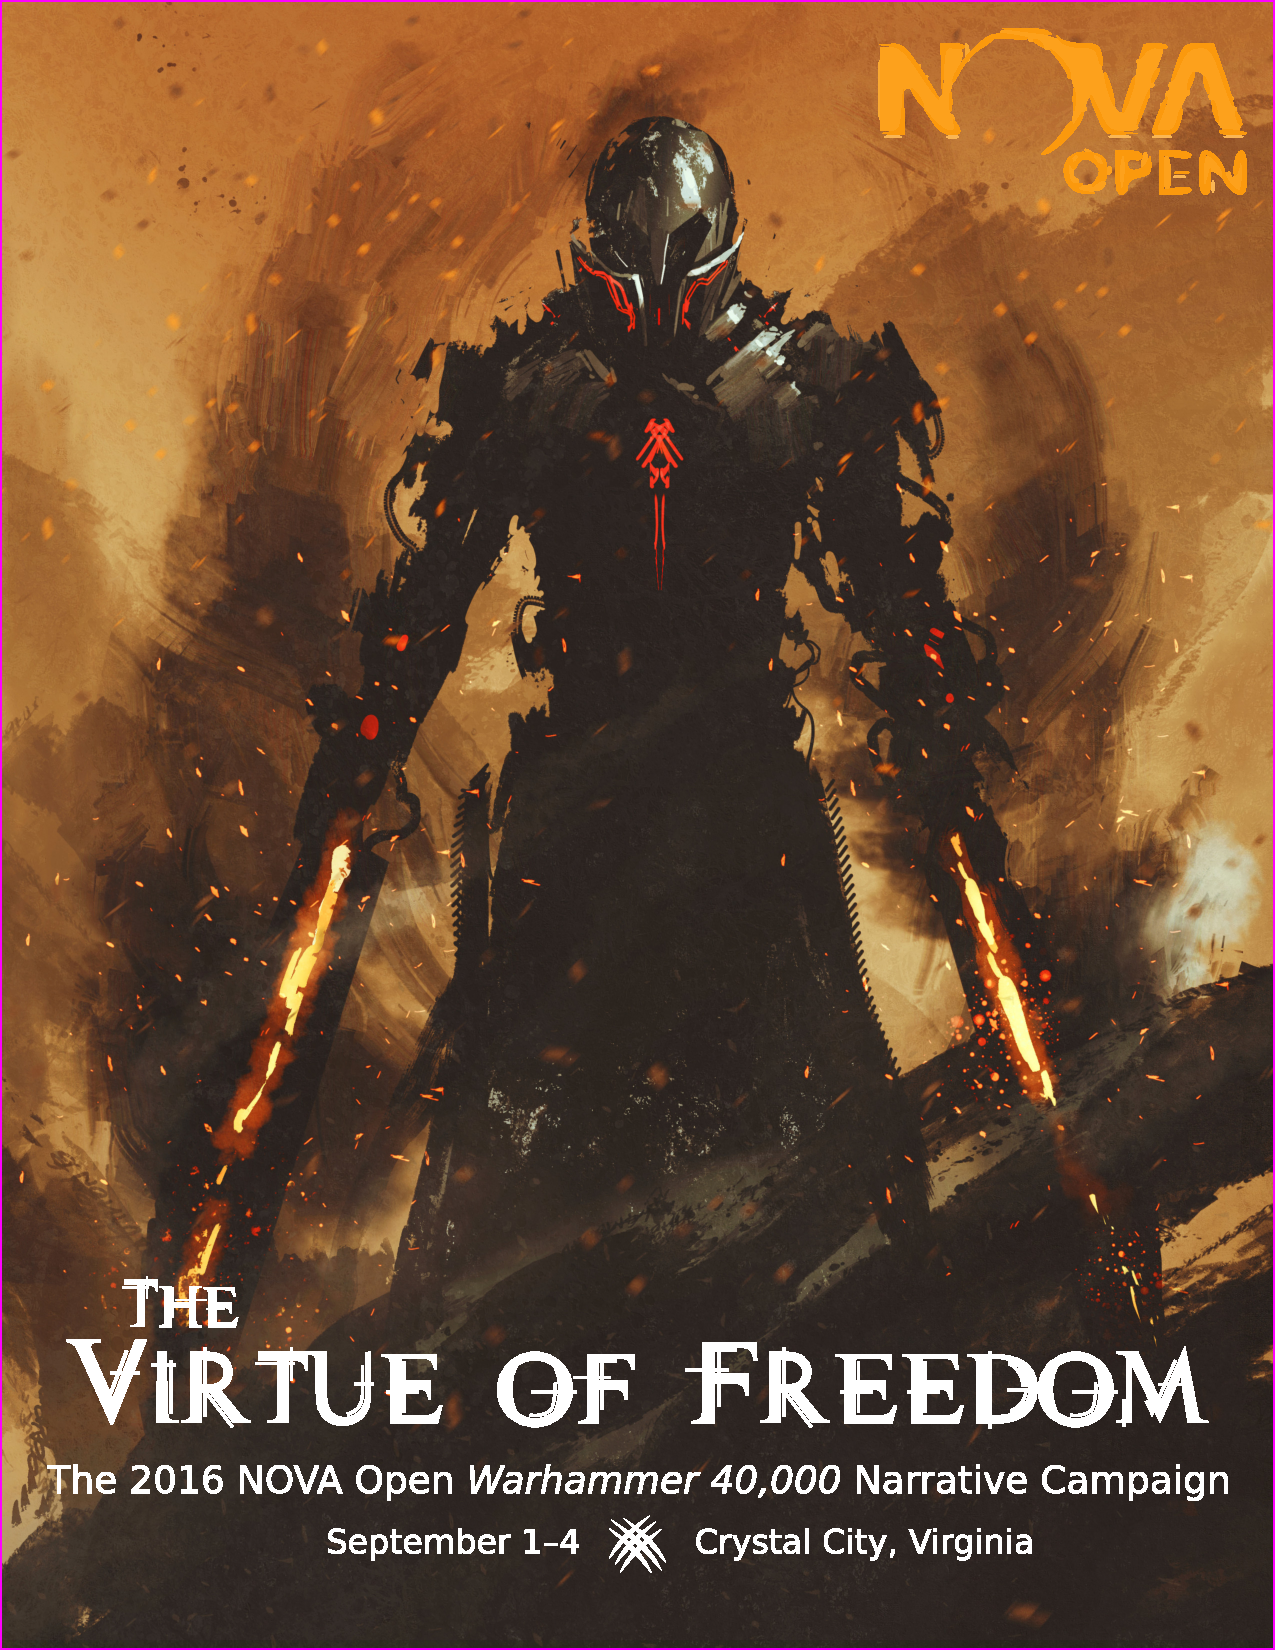
\includepdf[pages={1},fitpaper,offset=0cm 0cm]{art/cover/cover}
\pagebreak
\restorebackground

%%----------------------------------------------------------------------
%%----------------------------------------------------------------------
\begin{storyquotepage}  
  The Virtue society was founded amid chaos and bloodshed, war and
  betrayal.  Species fought species, worlds fought worlds, beings
  fought beings.  Violence was unceasing, ruthless.  The virtues and
  our adherence to them saved us.  Discipline, order, peace, these
  gave us a path forward.

  \bigskip And yet, along that path, we forgot one:\\
  The virtue of freedom.

  \bigskip - Sanctioned poet-in-exile Shossola,\\Commentaries
\end{storyquotepage}
%%----------------------------------------------------------------------
%%----------------------------------------------------------------------


%\setcounter{page}{1}
\chapter{Introduction}

Welcome to another year of the NOVA \textit{Warhammer 40,000}
Narrative!

The NOVA 40k Narrative is a high quality wargaming experience based on
an ongoing story in an original science fiction universe.  It is
team-centric, with players organizing into two alliances and
collectively making strategic decisions such as match pairings and
targets.  Most importantly, it is a narrative campaign, not a
tournament.  Stellar play and notable achievements are recognized, but
the focus is on social gaming with a strong narrative tilt.  Missions
aren't necessarily symmetric, and some of them aren't even fair.
Opponents also may or may not be working toward covert objectives of
which you're not even aware, or have a secret resource or stratagem
that they or their alliance won in earlier battles.  If your driving
motivation is competition and winning games, this event is not for
you.  If your main interest though is having fun, playing good games
with great people, and making your mark on a multi-year story built by
hundreds of fellow 40k gamers, then this is where you want to be
September 1--4, 2016.

Going into its fifth year, our player-created storyline continues with
The Virtue suffering the after-effects of its failed assault on Earth,
defeated by Humanity over the course of the previous events.  Whether
you're a new rookie or a returning veteran: Strap in, check your ammo,
and brace for impact---eons old, galaxy spanning civilizations don't
change easily.  Join us now for the 2016 NOVA 40k Narrative:

\bigskip
\centerline{
\includegraphics{art/title/title.pdf}}

\section{Updates}

This year's 40k Narrative is going to continue the things you love
about it.  But a number of changes and improvements are also being
made.  Primary gameplay updates of which to be aware include the
following:

\begin{itemize}
%\item The opposing sides in the story have broadened.

%\item Registration will be simplified and balancing of the sides
%  improved, with players signing up for the event as a whole and then
%  joining a side on opening night.

\item Codex-specific Narrative Supplements have been dropped.  They're
  too unwieldy to balance and maintain under Games Workshop's current
  hectic release schedule, as likely to imbalance armies as balance
  them, and skewed registration toward one or the other side in order
  to get specific boosts.

% \item Players will instead customize their armies through selecting a
%   Technical Skill, such as Field Medicine, Electronics, or
%   Assassination.  These will provide small, thematic in-game boosts;
%   notable advantages toward specific narrative mission objectives; and
%   a player-specific campaign progression.

\item Not everyone will be playing the same mission in each round,
  instead choosing from several options to meet the strategic needs of
  their side and to best match their style and army list.

\item Superheavy vehicles and gargantuan creatures with at most~9
  HP/Wounds are permitted.

\item An optional Quick Reaction Force detachment is made available to
  use in army lists.

\item New Fame and Infamy mechanics have been introduced.
\end{itemize}

\section{Release Schedule}

There are a number of significant components to the NOVA 40k
Narrative.  This player guide will be extended over the coming months
as they are developed, tested, and released.  The following milestones
are the latest by which you can expect details on those components.

\begin{center}  
\begin{tabular}{C{1.5in}L{5in}}
\rowcolor{LineColor}\textbf{\color{white} Date} & \multicolumn{1}{c}{\textbf{\color{white} Changes}}\\
  January 1 & Event schedule and basic army selection rules\\
  March 1 & Background story, campaign mechanics, and sample mission\\
  May 1 & Technical skills list, personal scoring, and painting contest rules\\
  July 1 & Public mission book, resources and stratagems samples\\
  September 1 & \textit{Game on!}\\
\end{tabular}
\end{center}


\section{Changelog}

This table summarizes what has been changed in each release of this document.

\begin{center}  
\begin{tabular}{C{1.5in}L{5in}}
  \rowcolor{LineColor}\textbf{\color{white} Date} & \multicolumn{1}{c}{\textbf{\color{white} Changes}}\\
August 8, 2016 & Full mission list, Fame and Infamy mechanics\\
  \rowcolor{LightGray}    March 31, 2016 & Background story and sample mission posted.  Minor rules about measuring to objective markers and a reminder of the standard startup sequence added.  QRF detachment tweaked to only grant choosing a trait from the BRB, and rerolling otherwise.\\
  January 31, 2016 & Schedule tweaked to better accommodate seminars.  Quick Reaction Force detachment made more restrictive.  Basic gameplay rules added (invisibility, rerollable 2+ saves, team games).\\
  \rowcolor{LightGray}  January 1, 2016 & Initial public release.
\end{tabular}
\end{center}


%%----------------------------------------------------------------------
%%----------------------------------------------------------------------
\chapter{Event Schedule}

There are two registration and participation tracks in the NOVA 40k Narrative:
\begin{itemize}
\item \textbf{Warlords.} Six amazing, storyful games, from Thursday
  night to Sunday mid-day, and war council meetings to make strategic
  decisions such as match objectives and pairings.

\item \textbf{Nightfighters.} Three great games on Thursday, Friday,
  and Saturday night.  This is a good option for players who want to
  participate in the 40k Narrative, but also play in NOVA 40k GT or
  other events.
\end{itemize}

The following table provides the detailed schedule for both tracks.

\begin{center}  
\begin{tabular}{C{0.75in}C{0.75in}C{2in}L{2.75in}}
\rowcolor{LineColor}\textbf{\color{white} Day} & \textbf{\color{white} Time} & \textbf{\color{white} Participants} & \multicolumn{1}{c}{\textbf{\color{white} Activity}}\\
  Thursday & 20:30 & Warlords \& Nightfighters & Joint Briefing \& Pairings\\
           & 21:30 & Warlords \& Nightfighters & \textbf{Battle Round 1}\\
\\
\rowcolor{LightGray} Friday     & 10:00 & Warlords                  & Alliance War Councils\\
\rowcolor{LightGray}            & 10:30 & Warlords                  & Pairings\\
\rowcolor{LightGray}            & 11:00 & Warlords                  & \textbf{Battle Round 2}\hfill\textit{(to 13:30)}\\
\rowcolor{LightGray}            & & & \\
\rowcolor{LightGray}            & 16:30 & Warlords                  & Joint Briefing\\
\rowcolor{LightGray}            & 17:00 & Warlords                  & Alliance War Councils\hfill\textit{(to 18:00)}\\
\rowcolor{LightGray}            & & & \\
\rowcolor{LightGray}            & 20:30 & Warlords \& Nightfighters & Joint Briefing \& Pairings\\
\rowcolor{LightGray}            & 21:30 & Warlords \& Nightfighters & \textbf{Battle Round 3}\\
\\
                     Saturday   & 10:00 & Warlords                  & Alliance War Councils\\
                                & 10:30 & Warlords                  & Pairings\\
                                & 11:00 & Warlords                  & \textbf{Battle Round 4}\hfill\textit{(to 13:30)}\\
                                & & & \\
                                & 16:30 & Warlords                  & Joint Briefing\\
                                & 17:00 & Warlords                  & Alliance War Councils\hfill\textit{(to 18:00)}\\
                                & & & \\
                                & 20:30 & Warlords \& Nightfighters & Joint Briefing \& Pairings\\
                                &       &                           & \emph{Paint Judging (tentative)}\\
                                & 21:30 & Warlords \& Nightfighters & \textbf{Battle Round 5}\\
\\
\rowcolor{LightGray}   Sunday   & 10:30 & Warlords                  & Joint Briefing\\
\rowcolor{LightGray}            & 11:00 & Warlords                  & Alliance War Councils\\
\rowcolor{LightGray}            & 11:30 & Warlords                  & Pairings\hfill\textit{(to noon)}\\
\rowcolor{LightGray} & & & \\
\rowcolor{LightGray}            & 13:00 & Warlords                  & \textbf{Battle Round 6}\hfill\textit{(to 15:30)}\\
\rowcolor{LightGray}            & 16:30 & Warlords \& Nightfighters & Joint Briefing: Outcomes!\hfill\textit{(to 17:00)}\\
\end{tabular}
\end{center}

%%----------------------------------------------------------------------
%%----------------------------------------------------------------------
\makeatletter\@openrightfalse
\chapter{Story So Far}
\@openrighttrue\makeatother

We pick up our tale in the future...

\bigskip
\begin{center}  
\begin{tabular}{L{6in}}
  \arrayrulecolor{LineColor}\hline\\
  {\it
  The Virtue is the greatest civilization ever arisen in the galaxy.
  More than a species, more than an empire, more than a philosophy; The
  Virtue is a way of being.  Its culture and technology
  are unsurpassed.  Its will is absolute.  The Virtue is perfect.

  \bigskip
  The Virtue \emph{was} perfect.

  \bigskip
  It has been two hundred years since The Virtue fought Humanity.  Their
  pacification forces were smashed, but at great cost to the human
  defenders.  Earth is a barren husk.  Its mighty war fleets have
  vanished, scattered to the solar winds if not lost entirely.  A paltry
  few survivors' colonies have integrated into the ignored, disordered, minor
  societies along the fringe worlds and outlaw regions at the edge of The Virtue's control,
  enduring as best they can
  in the shadow of the colossus.

  \smallskip
  The Virtue, for its part, has retreated into itself.  Effects of that
  failed conquest echo still, slowly rippling across the staid society.
  For the first time in millennia, murmurs of disquiet have been heard
  in the governance enclaves.  Questions flitter across the dataplane.
  How could a perfect society be defeated by such an unenlightened race?
  In a universe where everything is known, what could be unknown?

  \smallskip
  Spawned from this moral crisis, disparate elements on the perimeter of
  The Virtue's space have begun fomenting open rebellion.  Branding themselves
  the Coalition of the Free, their messages have appeared across
  message boards and even hastily graffitied in public spaces on the
  outer worlds, praising a new virtue:

  \bigskip
  \centerline{The virtue of freedom.}
  }
  \\
  \arrayrulecolor{LineColor}\hline\\
\end{tabular}
\end{center}

\section{The Past}

The~2016~40k Narrative continues the ongoing NOVA story of The Virtue
and Humanity.

\paragraph{NOVA 2012: First Contact.}  After a brush with global
nuclear war in~2194, humanity stepped back from the brink.  The
millennia-old dreams of scholars, tyrants, and preachers became a
reality as all the people of Earth finally set aside their
differences.  That peace was shattered a mere eighteen years later
when thousands of alien craft struck the planet without warning.
Millions died before any response could even begin.  Eventually though
a resistance formed.  Taking its last stand in Washington, D.C., the
defenders were dumbfounded when the invaders inexplicably retreated.

%\clearpage
\noindent\begin{minipage}[c]{(0.6\linewidth)-1em}%\vbox to 0pt{}
\paragraph{NOVA 2013: Cataclysm.}  Learning what they could from alien
captives and technology left behind, humanity strove to rebuild and
prepare.  Their caution was well founded: In~2312, one hundred years
to the day of the first invasion, the invaders struck again.  Against
much improved resistance and plagued by doubts, they once more though
faltered even as millions died.  Faced with defeat, their commander
rammed his flagship into Earth in a final ignominious gesture,
igniting its antimatter cores in the planetary mantle.  The blast and
shockwaves killed billions, with billions more lost in catastrophic
aftereffects.  Humanity survived merely through those few population
centers shielded enough to outlast the trauma.

\bigskip
\paragraph{NOVA 2014: Descension.} Regrouping in the aftermath,
humanity began a two-pronged offensive.  Space fleets began pushing
outward from Earth, learning much about the invaders and from where
they had come.  Forces on Earth meanwhile attempted to cleanse the
planet of the numerous aliens still fighting on.  This fight however
was doomed.  The planet had simply sustained too much damage, and the
numerous invaders still extant on the surface were only working to
further its destruction.  Eventually the cold truth became clear and
inevitable: The Earth was truly lost.
\end{minipage}\hfill%
\begin{minipage}[c]{0.4\linewidth}%\vbox to 0pt{}
  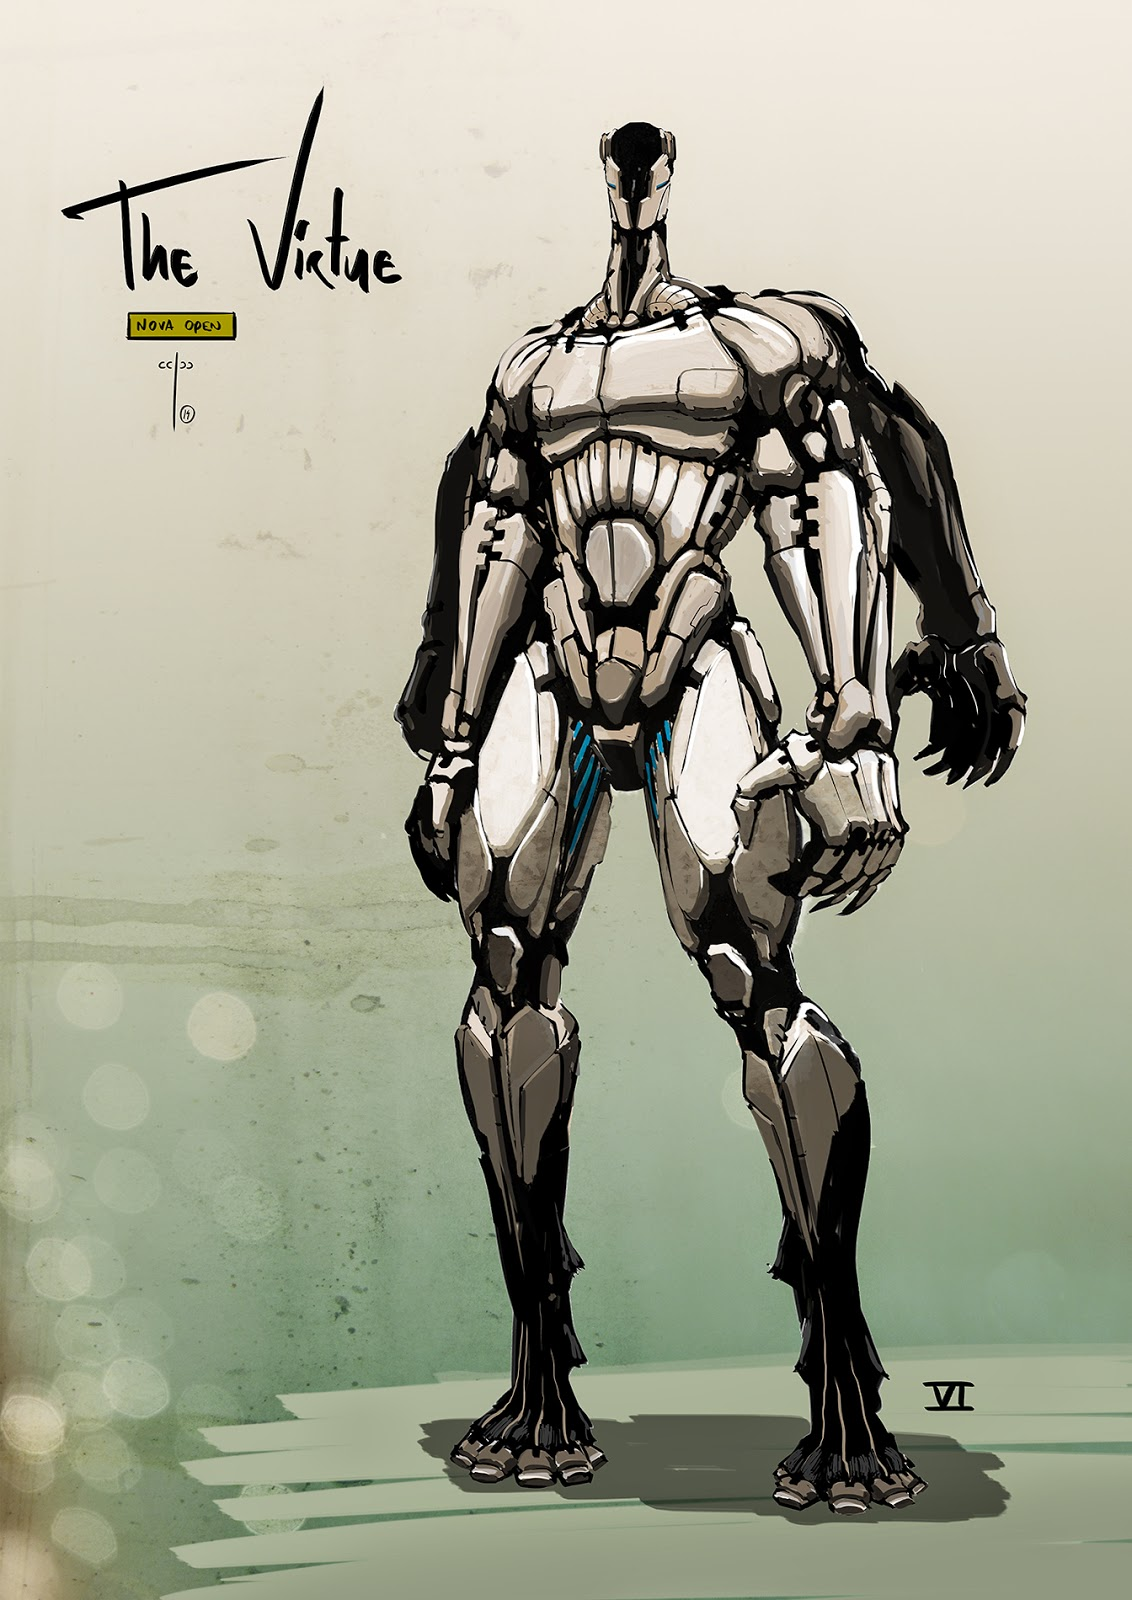
\includegraphics[width=\linewidth]{art/characters/virtue-warrior.jpg}
\end{minipage}

\paragraph{NOVA 2015: Ascension.}  Building on their successes,
humanity's remaining military focused their efforts on the war in
space.  A massive invader space station was discovered and captured,
yielding access to the Bend gates through which they warped time and
space to travel the void.  Meanwhile, ground forces fought to rescue
and protect what remnants of Earth's remaining population they could.
Although a tremendous evacuation was enacted, its scale was tragically
dwarfed by all those necessarily left behind.  Their hand forced by
the ongoing fighting, the survivors waited as long as they could
before closing and destroying the Bend gate inbound to Earth before
launching on their exodus through the outward gate into the stars...

\section{The Virtue}

The alien invaders that beset Earth in~2212 were eventually revealed
as warriors of The Virtue.  For thousands of years The Virtue have
ruled much of the galaxy, encompassing innumerable worlds and species.
Built on fundamental, inarguable virtues and morals, over millenia the
tenets of their society have progressed to become part of their
collective genetic makeup itself.  The Virtue society can do no wrong,
and its citizens need not question if they might do wrong in following
its dictates.

As such, none of The Virtue warriors encountered in the fighting over
Earth had ever questioned their task.  For all of known history The
Virtue had stood in judgement over all the fledgeling races of the
galaxy.  As those species reached the threshold of relevance, The
Virtue applied a standard protection and inclusion protocol: Were they
a destructive cancer to be eliminated, or a desirable new element to
be incorporated into The Virtue?  Humanity was simply found wanting,
no further explanation needed.

But those colossal, four-armed warriors encountered on Earth are but
one face of The Virtue, just one of its militaries tasked with
pacifying young races.  The Virtue society is truly vast, and deep
within its governance structures another conclusion had been derived
from the protocols.  From that initial crack, the events at Earth have
slowly emerged as a growing fault line in the very foundations of The
Virtue society.  Never before had The Virtue been turned back from its
objectives, least of all by such an insignificant young race as
Humanity.  For those that have truly considered the implications, the
sheer outrageousness of the defeat calls into question the very
essence of The Virtue.  Eons-old civilizations don't fall often or
easily, but when they do, it comes from doubts such as these.

\section{The Free}

Two centuries later, those doubts have flickered into wisps of open
dissent.  On a far flung edge of The Virtue's territory, a group
labeling itself the Coalition of the Free has developed as if from
nowhere and taken increasingly provocative actions.  It began on the
public forums of the dataplane, messages citing discouraged texts and
raising questions from hijacked sockets beamed into from unrecognized
space.  Emboldened by faint stirrings of doubt, Coalition-sponsored
covert meetings began appearing on worlds of The Virtue themselves,
disseminating their message and recruiting to their beliefs.
Recently, the most brazen cells have shockingly defaced government
buildings and even sabotaged pacification assets.

Operating within the strictures of their philosophy and being, local
Virtue officiants have been unable to truly process and address these
events.  Most hazily interpret the Coalition of the Free as outside
attackers feared to be on the verge of invading The Virtue space.
Although almost wholly unprecedented, this is at least a largely
understandable concept.  Deeper, darker corners of The Virtue though
better understand the true threat.  Worse, they suspect and fear that
the Coalition has been helped by traitorous elements within the
government.  Elements that might even explain mysterious aspects of
the defeat at Earth.

Within the Coalition of the Free itself, hopes and passions run
rampant as wildfire.  Twinned rumors circulate among its cells.  One
tells of the discovery of a mighty weapon with which to fight The
Virtue.  Another posits an opportunity in the near future to make a
daring strike at a very pillar of The Virtue's control in the
region.  True or false, the whole of its decentralized structure
buzzes with activity and preparation...

\section{The Future}

The NOVA 2016 40k Narrative begins at this moment on the precipice,
and players must choose a side:

\begin{center}
\begin{minipage}[c]{1in}
  \fbox{
\includegraphics[width=\linewidth]{art/icons/free.pdf}}
\end{minipage}%
\hspace{2em}%
\begin{minipage}[c]{4in}
  Fight for \textbf{Humanity} as a leader and instigator of the
  Coalition of the Free, striving to capture the rumored weapon and
  strike at The Virtue to preserve your race and release many others
  from its oppressive grip.
\end{minipage}

\bigskip
  
\begin{minipage}[c]{4in}
  Command a military of \textbf{The Virtue}, directing a pacification
  force dispatched to uncover the traitor, quell rebellion, hunt down
  outside agitators, and restore peace and order by smashing the
  Coalition of the Free decisively.
\end{minipage}%
\hspace{2em}%
\begin{minipage}[c]{1in}
  \fbox{
\includegraphics[width=\linewidth]{art/icons/virtue.pdf}}
\end{minipage}
\end{center}

%%----------------------------------------------------------------------
%%----------------------------------------------------------------------
%\begin{storyquotepage}  
%  Even the smallest of daggers can cause the\\gravest of wounds if they
%  come from behind.
%
%\bigskip
%- Attribution lost,\\Chronicles of Foundation,\\restricted historical draft
%\end{storyquotepage}

\makeatletter\@openrightfalse
\chapter{Army Selection}
\@openrighttrue\makeatother

Each player must prepare two army lists:

\begin{itemize}
\item \textbf{Campaign Force.} For your individual battles, the
  majority of the campaign.\hfill\textit{Up to 2000 points.}

\item \textbf{Strike Force.} For your team games, of which there will
  be at least one.\hfill\textit{Up to 1000 points.}
\end{itemize}

Both army lists must be battle forged.  No model with more than~9 hull
points or wounds is permitted.  Superheavy vehicles and gargantuan
creatures are otherwise allowed.

The strike force list need not be a subset of the campaign force list,
but cannot include any factions not utilized in the campaign force
list.  As detailed below, in team games you will have your own
warlord, and your units will count as allies of convenience to those
of your partner(s), regardless of factions.

No other requirements or constraints are placed on detachments,
formations, or force organization. An optional Quick Reaction Force
detachment is made available for this event, described below.

\section{Sources}

Forgeworld units and armies eligible for standard \textit{Warhammer
  40,000}, i.e., not \textit{Apocalypse}, are permitted. Units and
armies from Forgeworld's Horus Heresy \textit{Age of Darkness} books
are also permitted.

All up-to-date, official \textit{Warhammer 40,000} army sources are
permitted that are available in current publication. This does include
White Dwarf entries, which are available via back issues, and current
campaign books. It does not include limited edition dataslates and
formations, e.g., those included in mega-bundles. Contact the
tournament organizer(s) beforehand about any questions. Remember that
you must have all sources on hand, electronically or digitally.

For any codex or supplement re-released within two weeks preceding the
event, you may choose whether to use the old or new edition. You may
not use both editions of a single source within the event.

\section{Models}

Models must be WYSIWYG, but identifiable and thoughtful conversions
and proxies are welcome. Indistinguishable or confusing proxies are
not acceptable.  Contact the organizer(s) beforehand for any
questions.

In addition, models need not be painted, but is \textit{very strongly}
recommended in order to not impair the experiences of all other
participants.  A painting component will be applied to personal scores
to reward finished armies, following the standardized NOVA metrics.


\clearpage
\section{Quick Reaction Force}

Players may optionally employ a Quick Reaction Force detachment in
their army lists, defined as follows.

\subsection{Force Organization}

An army may only contain a single Quick Reaction Force detachment.
All units in the detachment must have the same faction, or no faction.
The detachment is comprised of the following battlefield roles.

\begin{center}
\begin{tabular}{C{0.75in}C{0.75in}C{0.75in}C{0.75in}C{0.75in}C{0.75in}}
\rowcolor{LineColor}\textbf{\color{white} HQ}	& \textbf{\color{white} Troops}	& \textbf{\color{white} Elites}	& \textbf{\color{white} Fast Attack}	& \textbf{\color{white} Heavy Support}	& \textbf{\color{white} Lords of War}\\
1--2	& 2--6	& 1--4	& $\star$	& $\star$	& 0--1\\
\end{tabular}
\end{center}

A Quick Reaction Force detachment must include one Fast Attack and one
Heavy Support choice. It may include up to three selections in one of
those roles, but must contain one and only one selection in the other
role. I.e., the detachment must adhere to one of the following
options:

\begin{itemize}
\item 1--3 Fast Attack and 1 Heavy Support
\item 1 Fast Attack and 1--3 Heavy Support
\end{itemize}

As usual, dedicated transports are not counted toward these quantity limitations.

\subsection{Command Benefits}

The following advantages are granted for utilizing this detachment:

\begin{itemize}
\item \textbf{Objective Secured.} All scoring units in this detachment
  except superheavy vehicles and gargantuan creatures gain Objective
  Secured. A unit with this special rule controls objectives even if
  an enemy scoring unit is within range of the objective marker,
  unless the enemy unit also has this special rule.

\item \textbf{QRF Commander.} If this detachment is your primary
  detachment, instead of rolling a random warlord trait you may choose
  a warlord trait from the tables in the main \emph{Warhammer 40,000}
  rulebook.  If you wish to use a different table of warlord traits,
  i.e., from a codex, then you must roll a random trait, but may
  reroll the result.

\end{itemize}

%%----------------------------------------------------------------------
%%----------------------------------------------------------------------
\makeatletter\@openrightfalse
\chapter{Gameplay Rules}
\@openrighttrue\makeatother

This section defines the basic gameplay rules applied in the 40k Narrative.

\section{Core Rules}

The following rules apply to all games in the NOVA 40k Narrative.

\paragraph{Time Limits.}
Matches are scheduled for~2.5 hours, but players may take more time as
long as they mutually agree to do so.  Please discuss and agree to
play long or not at the start of each match, or at least well before
the time limit, so that there are no assumptions or mismatched
expectations.  This flexibility ensures that players may participate
in seminars and other NOVA events without hindering their Narrative
experience, but have the option to play at a relaxed pace if they have
no schedule constraints.  Results must be submitted at least half an
hour before the next activity on the Narrative schedule.

\paragraph{Invisibility.}
The Invisibility psychic power is amended to be:

\begin{center}  
\begin{tabular}{L{6in}}
\arrayrulecolor{LineColor}\hline\\
  \emph{Invisibility} is a blessing that targets a single friendly unit
  within 24". While the power is in effect, enemy units shooting at the
  target unit do so at BS 1, and in close combat will only hit models of
  the target unit on To Hit rolls of 5+.\\
\\
\arrayrulecolor{LineColor}\hline\\
\end{tabular}
\end{center}

\paragraph{Rerollable 2+ Saves.}
For any failed 2+ save that may be rerolled, the reroll only succeeds on a 4+.

\paragraph{Objective Markers.}
Standard objective placement constraints apply in setting up a game
unless noted otherwise by a specific mission.  Objective markers may
be controlled or contested by models/units up to 3" horizontally from
the side edge of the marker and 6" vertically from its bottom
face. Objective markers should all be the same size (typically
equivalent to a 40mm base).


\section{Team Rules}

The rules in this section apply to team games in the 40k Narrative.

\paragraph{Separate Allies.}
All players in a team field their strike force lists as separate
armies. Regardless of factions, teammates consider their
  partners' units and models to be allies of convenience to their own
  army.  In addition, all players on a team nominate a warlord for
themselves as usual.
%, thus a doubles pair would have two warlords in play.

\paragraph{Warp Storm Table.}
Results rolled by a player on the Warp Storm table (\emph{Codex: Chaos
  Daemons}) do not affect their teammates' armies and models unless
specifically dictated by the table, i.e., other Chaos Daemons or
marked Chaos Space Marines.

\paragraph{Psychic Phase.}
In the psychic phase, a single D6 is rolled by the current team to
determine the base warp charge from which each player on both teams
generates their own individual pools, applying the usual rules to
their own models. Players all use their own warp charge pool;
teammates cannot combine or share warp charge. Any opposing player
with models on the table may attempt to deny the witch, caveat that if
a specific unit of enemy models is targeted, their player alone may
attempt to block the spell.

\paragraph{Single Army.}
For all other gameplay purposes the combined forces of a team are
considered a single army comprised of multiple detachments, and the
team considered a single player for all rules except when specifically
distinguished by the missions here. How units belonging to different
players in a team interact are thus governed by the rules for allies
of convenience, on page 126 of the main \emph{Warhammer 40,000}
rulebook.  Being a single army also entails a number of other rules,
including:
\begin{itemize}
\item Units may not shoot at close combats even if none of their player's
units are engaged.

\item Teams are not eliminated unless there are no models of any member on
the table.
\end{itemize}



\section{Startup Sequence}

The start of each game proceeds as follows unless the mission notes
otherwise:

\begin{enumerate}\shortlist
\item Clarify terrain and mission rules

\item Share and clarify army lists

\item Determine warlord traits, then psychic powers, and then other
  pre-game effects and choices

\item D6 roll off to select deployment zones

\item Place primary objective markers

\item D6 roll off to choose first or second deployment

\item Deploy main armies in that order

\item Deploy any Infiltrators (pg. 167)

\item Secretly choose and record secondary objectives from the options
  listed for the mission

\item Make any Scout redeployments (pg. 171)

\item Reveal secondary objectives and any related selections or marker
  placements as directed

\item First to deploy chooses to play first or second

\item Seize the Initiative roll, if desired and permitted

\item \emph{Battle!}
\end{enumerate}

% %%----------------------------------------------------------------------
%%----------------------------------------------------------------------
\makeatletter\@openrightfalse
\chapter{Campaign}
\@openrighttrue\makeatother

Hello

%%----------------------------------------------------------------------
%%----------------------------------------------------------------------
\makeatletter\@openrightfalse
\chapter{Missions}
\@openrighttrue\makeatother

\newcommand{\missionicon}{\raisebox{-8pt}[6pt][-2pt]{\protect
\includegraphics{art/icons/mission.pdf}}}
\newcommand{\single}{\hfill~\missionicon}

Each round of the campaign, as part of their strategic decision
making, the two alliances will alternate putting forward a player and
a mission chosen from those in this section.  The other team will then
respond with an opponent and a table for the match.  These pairings
will be conducted within groups of~8 per side, determined by win/loss
ranks.  Missions marked with a~\resizebox{!}{4pt}{\missionicon}~may only be selected once
within each group.

\textbf{Some missions need special models, such as convoy vehicles,
  shuttlecraft, and VIPs.  All matches will also use a set of
  civilians.  These will all be provided.}

\section{Scoring}

Match results are determined by scoring primary, secondary, and
tertiary objectives.  All missions use the same tertiary and secondary
objectives, explained below.  Individual missions define their primary
objective(s).  \underline{No more than a total of~9 victory points may
  be earned for primary objectives,}~6 for secondary objectives, and~5
for tertiary objectives, for a total of no more than~20 victory points
possible in a match.  The winner is the player with more victory
points at game end, or a draw if they earned equal amounts.
  
\section{Standard Mission Rules}

The following special rules are applied to each mission unless noted
otherwise.

\vspace{-2pt}
\paragraph{Easy Recon.}  Players add~+1 to their roll to
choose first or second deployment for each superheavy vehicle or
gargantuan creature in the opposing army.

\vspace{-2pt}
\paragraph{Reserves.} As defined on page~135 of the main
\emph{Warhammer 40,000} rulebook.

\vspace{-2pt}
\paragraph{Seize the Initiative.} As defined on page~132 of
the main \emph{Warhammer 40,000} rulebook.

\vspace{-2pt}
\paragraph{Variable Game Length.} As defined on page~133 of
the main \emph{Warhammer 40,000} rulebook.

\vspace{-2pt}
\paragraph{All In.}  Units/models in reserve at game end count
as completely destroyed/removed as a casualty.

\section{Tertiary Objectives}

The following common tertiary objectives apply in each mission.
\underline{At most~5 total victory points may be}
\underline{earned by a player across all of the tertiary objectives.}

\begin{itemize}[noitemsep]
\item \textit{Victory Through Attrition.}  Score~1 victory point for
  every~2 unsaved hull points or wounds suffered by an opposing
  superheavy vehicle or gargantuan creature through any means,
  including explosions and other indirect effects.  These points are
  earned at the end of any phase in which such damage occurs, and thus
  include any repaired or regenerated later.

\item \textit{Slay the Warlord.}  If your opponent's Warlord or a Lord
  of War character of theirs has been removed as a casualty or is
  falling back at the end of the game, score~2 victory points.

\item \textit{Linebreaker.}  Score~2 victory points if a model from
  any friendly scoring unit is completely within 12'' of your
  opponent's table edge.

\item \textit{First Blood.}  As defined on page~133 of the main
  \emph{Warhammer 40,000} rulebook.

\item \textit{Special Conditions.}  Any unit, faction, formation, or
  other special rules granting victory points to either player are
  considered tertiary objectives and are included within the~5 point
  cap.
\end{itemize}

%%----------------------------------------------------------------------
%%----------------------------------------------------------------------
\input{mission-list}
\newcommand{\missiontitle}[1]{\clearpage\section{#1}}
\newcommand{\missionheading}[1]{\subsection{#1}}
\newcommand{\missionsubheading}[1]{\paragraph{#1}}
\setlength{\headingspacing}{0pt}

%%----------------------------------------------------------------------
%%----------------------------------------------------------------------
%%%----------------------------------------------------------------------
%%----------------------------------------------------------------------
\missiontitle{Mission: Brushfire}

\smallskip
\teaser{Both sides fight to control ground amid the sudden open rebellion.}
\bigskip

\begin{tablesetup}

  \dawnofwar

  \smallskip%
  Place one primary objective marker at table center.  Beginning with
  the winner of a~D6 roll off, both players alternate placing one
  primary objective marker and then a second, for a total of~5 on the
  board once setup is complete.  These markers may be placed anywhere
  on the board within the standard rules.
\end{tablesetup}

%%----------------------------------------------
\begin{missionrules}
\nightfighting
\end{missionrules}


%%----------------------------------------------
\begin{scoring}
  
\begin{primaries}

  Before any Scout redeployments, both players secretly choose one of
  the following primary scoring mechanisms for themselves:

  \begin{itemize}
  \item {\textit{Continuous.}} Beginning with Turn~2, score~1 victory
    point at the end of each of your player turns for each primary
    objective marker you control.
  
  \item {\textit{End Game.}} At game end, score~3 victory points for
    each primary objective marker you control.
  
  \end{itemize}

  This selection is declared along with the choice of secondary
  objective, below, after Scout redeployments.  Remember that
  \underline{no more than 9 victory points may be earned toward
    primary objectives}.

\end{primaries}

\begin{secondaries}
  \interrogation
  \civilians
%  \breaktheirback
%  \securepositions
\end{secondaries}

\end{scoring}


%%----------------------------------------------------------------------
%%----------------------------------------------------------------------
\clearpage
\section{Secondary Objectives}

In each match the players must choose a secondary objective for
themselves from the following list.  \underline{At most~6 total
  victory points may be earned by a player toward their secondary
  objective.}

\begin{itemize}[leftmargin=2em]
\assassination

\chosenground

\controlthefield

\frontline

\hullbreaker

\interrogation

\meatgrinder

\seekanddestroy

\seizeground

\end{itemize}


%%----------------------------------------------------------------------
%%----------------------------------------------------------------------
\clearpage
\section{Civilians}

The campaign's conflict does not occur in a vacuum---all games will
include civilians to be slaughtered or saved as the players wish.
Before selecting deployment zones, roll off and alternate in that
order placing~3 civilians each (both teammates do so in doubles
games).  They must be placed outside both deployment zones, at least
12'' from each other and at least 6'' from table edges.

  \begin{center}    
  \begin{tabular}[t]{O{0.75in}ccccccccF{.25in}F{1in}E{2in}}
    & {\bf WS} &  {\bf BS} & {\bf S} & {\bf T} & {\bf W} & {\bf I} & {\bf A} & {\bf Ld} & {\bf Sv} & {\bf Type} & {\bf Special Rules}\\
\hline
    {\bf Civilian} & 1 & - & 2 & 2 & 1 & 3 & - & 4 & 6+ 6++ & Infantry & Neutral NPC\\
  \end{tabular}
  \end{center}

  \label{rule:neutral-npc}
  \hfill
  \begin{minipage}{6in}
    \missionsubheading{Neutral NPC.} Units of either player may join a
    neutral NPC following the rules for independent characters.  Once
    joined, the NPC is considered a model of that player's army until
    the unit is eliminated or detaches from the NPC.  It may embark in
    transports and buildings while part of a unit; a unit cannot
    detach while embarked and leave an NPC behind embarked.  The NPC
    never moves on its own, including to join or leave units.  Players
    may shoot and assault unattached NPCs as though they were enemy
    models.  Models in an attached unit may Look Out, Sir! to protect
    the NPC from wounds allocated to it, and the NPC may be used to
    Look Out, Sir! and protect another model.  NPCs are not scoring
    and never count toward any mission objectives, including but not
    limited to kill points and controlling objective markers, even
    while joined to a unit.
  \end{minipage}
  \hfill\hbox to 0pt{}


\missionheading{Fame and Infamy}

The fate of civilians critically determines each army's reputation,
measured by the number of points earned toward fame and infamy.  Both
of these are tracked, and the final leader for each awarded a small
prize.

\missionsubheading{Wanton Slaughter.}  Any attack that eliminates a
civilian earns the attacking player~2 infamy points.

\missionsubheading{Meat Shields.}  If a civilian joined to a unit is
the first model removed when the unit is targeted by shooting, psychic
attacks, or in a round of close combat, or if a civilian is removed
after being used to Look Out, Sir! for another model in an attached
unit, then the unit's player earns~1 infamy point.

\missionsubheading{Heroes of the People.}  At game end, each civilian
attached to a unit earns that player~4 fame points.

\missionsubheading{Safe Haven.}  At game end, each unattached civilian
wholly inside a player's deployment zone earns that player~2 fame
points.

\missionsubheading{Black and White.}  Fame and infamy are exclusive of
each other.  After each match, only the greater of the player's fame
or infamy will be added to their respective running total, after
subtracting the lesser.


%%----------------------------------------------------------------------
%%----------------------------------------------------------------------
\missiontitle{Mission: Comms Facility\single}

\teaser{You must claim---or at least deny the enemy---a critical
  communications facility!}

\begin{tablesetup}

  \hammerandanvil

  \smallskip%
  Before choosing deployment zones, place a Comms Facility on the
  board.  Both players nominate a location within 12'' of table center
  where the building can be placed without overlapping any terrain (or
  as close as is possible to do so).  Randomly select one of the
  locations and place the Comms Facility there.

  \begin{center}    
  \begin{tabular}[t]{rcccccL{3in}}
    & {\bf BS} &  {\bf F} & {\bf S} & {\bf R} & {\bf HP} & {\bf Special Rules}\\
    {\bf Comms Facility} & - & 12 & 12 & 12 & 3 & Small Building, Capacity 5, 1 Access Point\\
  \end{tabular}
  \end{center}

%  \hfill
%  \begin{minipage}{6in}
%  \end{minipage}
%  \hfill\hbox to 0pt{}

  \noindent
  \begin{minipage}[t]{\linewidth-(2.5in+1em)}\vbox to 0pt{}
    \hspace{1em} If the building is destroyed or explodes, do not
    remove the model but treat it as rubble from then on (dangerous
    terrain, 5+ cover).  Both the building and its rubble act as an
    objective marker.

    \hspace{1em} Next place~4 primary objective markers each~12'' from
    the Comms Facility directly toward each table edge but at least
    6'' from that table edge, as the example to the right shows.

    \hspace{1em} The comms facility is not part of either army and
    never counts toward any secondary or tertiary objectives.


    \begin{missionrules}
      \bigskip
      There are no rules specific to this mission.
    \end{missionrules}

  \end{minipage}\hfill
  \begin{minipage}[t]{2.5in}\vbox to 0pt{}
  
\includegraphics[width=\linewidth]{missions/comms-placement}
  \end{minipage}

\end{tablesetup}

%%----------------------------------------------

%%----------------------------------------------
\begin{scoring}  
\begin{primaries}

  Each player earns victory points by the state of the Comms Facility
  at game end:

\begin{center}  
  \begin{tabular}{C{1in}C{1in}C{1in}C{1in}C{1in}}
\rowcolor{LineColor} {\color{white}\bf Destroyed} & {\color{white}\bf Wholly Intact} & {\color{white}\bf Player Controls} & {\color{white}\bf Opponent Controls} & {\color{white}\bf Victory Points}\\
No & Yes & Yes & No  & 5\\
\rowcolor{gray!25} No & No  & Yes & No  & 3\\
No & Yes & No  & Yes & 0\\
\rowcolor{gray!25} No & No  & No  & Yes & 1\\
No & Yes & No  & No  & 3\\
\rowcolor{gray!25} No & No  & No  & No  & 2\\
Yes & No & Yes & No  & 3\\
\rowcolor{gray!25} Yes & No & No  & Yes & 1\\
Yes & No & No  & No  & 2\\
  \end{tabular}
\end{center}

A unit on the roof of the building trumps all units on the exterior
for control of the building.  A unit embarked in the building trumps
units on the roof and exterior.

In addition, each primary objective marker controlled at game end
yields~1 victory point.

%\underline{Remember that no more than~9 victory points may be earned
%  toward primary scoring.}

\end{primaries}
\end{scoring}

%%----------------------------------------------------------------------
%%----------------------------------------------------------------------
\missiontitle{Mission: Convoy\single}

\teaser{The supplies in this vehicle are desperately needed on the
  front line, see that they get through!}

\begin{tablesetup}

  \dawnofwar

  \smallskip%
  Before any deployment begins, each player gains a Bulldog Transport
  for their army:

  \begin{center}    
  \begin{tabular}[t]{rcccccL{3in}}
    & {\bf BS} &  {\bf F} & {\bf S} & {\bf R} & {\bf HP} & {\bf Special Rules}\\
    {\bf Bulldog Transport} & - & 11 & 11 & 10 & 3 & Smoke Launchers (4), Transport (6), Advanced Repair Systems, Tank\\
  \end{tabular}
  \end{center}

  \hfill
  \begin{minipage}{6in}
    \missionsubheading{Advanced Repair Systems.} If the vehicle is
    immobilized at the start of its movement, roll a~D6.  On a~4+ it
    is no longer immobilized, and may immediately move as normal.  It
    does not regain any hull points lost.  If the roll is failed then
    the vehicle may move 3'' as it attempts to lurch back to life.
    This roll may be taken every turn until successful.
  \end{minipage}
  \hfill\hbox to 0pt{}

  \bigskip The Bulldogs may not be held in reserve and must deploy
  wholly within 6'' of the player' table edges.  They do not count
  toward any secondary objective but do count toward First Blood and
  Linebreaker.
\end{tablesetup}

%%----------------------------------------------
\begin{missionrules}

\bigskip
There are no rules specific to this mission.

\end{missionrules}


%%----------------------------------------------
\begin{scoring}  
\begin{primaries}

  At the end of the first movement phase in which a player's Bulldog
  is fully within their opponent's half of the table, the controlling
  player gains~2 victory points.  At the end of the first movement
  phase in which a player's Bulldog is fully within their opponent's
  deployment zone, the controlling player gains~1 victory point.  At
  game end, players earn~3 victory points if their Bulldog has not
  been destroyed.  They also earn~1 victory point for each hull point
  removed from their opponent's Bulldog.

%\underline{No more than~9 victory points may be earned by primary objectives.}

\end{primaries}
\end{scoring}

%%----------------------------------------------------------------------
%%----------------------------------------------------------------------
\missiontitle{Mission: Shuttle Crash\single}

\teaser{A courier shuttle has been shot down, you must seize the pilot
  and their databanks!}

\begin{tablesetup}

  \dawnofwar

  \smallskip%
  After all deployment concludes, randomly determine a table corner.
  Place a flying shuttle marker~12''x12'' from that corner, adjusting
  its position by the minimum distance necessary toward table center
  to not overlap models or impassible terrain.  Models may move under
  the shuttle model and over or onto its base.
\end{tablesetup}

%%----------------------------------------------
\begin{missionrules}
\vspace{-1.5em}%
\noindent%
  \begin{minipage}[t]{\linewidth-(1.75in+1em)}\vbox to 0pt{}
    \textbf{Shuttle Crash.} At the start of game turn~2, either player
    rolls a~D6.  On a~1--2 the shuttle marker scatters toward the
    diagonally opposite table corner, on a~3--4 it scatters toward the
    center of one of the farther opposing table edges, and on a~5--6
    it scatters toward the center of the other farther opposing table
    edge, as shown to the right. The shuttle scatters~3D6 in that
    direction and becomes crashed.

    \smallskip\hspace{1em} Next, place~4 debris markers,~12+2D6'' from
    the shuttle's final position toward each of the~four table
    corners, rolling the distance for each separately.

    \smallskip\hspace{1em} Neither shuttle nor debris will crash onto
    impassable terrain.  Adjust their final positions by the minimal
    necessary distance to prevent this.
  \end{minipage}\hfill
  \begin{minipage}[t]{1.75in}\vbox to 0pt{}
  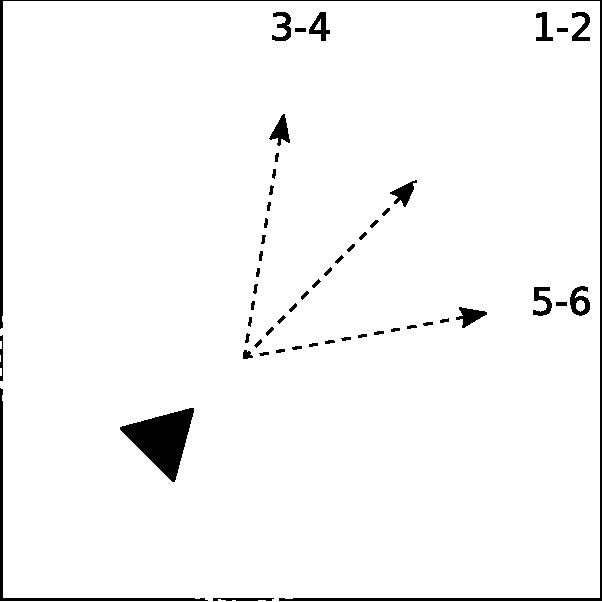
\includegraphics[width=\linewidth]{missions/shuttle-scatter}
  \end{minipage}

  \smallskip Any non-vehicle models under the shuttle or debris
  markers' final positions must pass an initiative test or take a
  wound. Vehicles under such a marker take an~S8 hit on their side
  armor.  Cover saves are not permitted for either but armor and
  invulnerable saves are.  Surviving models are displaced the minimum
  necessary distance to not overlap any marker, model, or impassable
  terrain.

  \smallskip The crashed shuttle and debris act as objective markers,
  dangerous terrain, and give a~5+ cover save.

  \missionsubheading{Wounded Pilot.} At the end of the first movement
  phase in which at least one non-vehicle model is in base contact
  with or on the crashed shuttle marker, the current player places a
  Pilot in base contact with any such model of their choice.  The
  Pilot joins that unit unless forbidden by the latter's rules.

  \begin{center}    
  \begin{tabular}[t]{O{0.75in}ccccccccF{.25in}F{1in}E{2in}}
    & {\bf WS} &  {\bf BS} & {\bf S} & {\bf T} & {\bf W} & {\bf I} & {\bf A} & {\bf Ld} & {\bf Sv} & {\bf Type} & {\bf Special Rules}\\
\hline
    {\bf Pilot} & 3 & - & 3 & 3 & 2 & 2 & - & 7 & 5+ 6++ & Infantry & Neutral NPC\\
  \end{tabular}
  \end{center}

  \hfill
  \begin{minipage}{6in}
    \missionsubheading{Neutral NPC.} See
    page~\pageref{rule:neutral-npc} of this mission book.
  \end{minipage}
  \hfill\hbox to 0pt{}

  % \missionsubheading{Debris.}  Any uncontested debris marker that
  % begins the movement phase in base contact with at least two infantry
  % models from a single unit may be carried up to~6'' by those models
  % as they move, ending the move in base contact with both models.
  % Designate two before moving if there are multiple models in base
  % contact.  No unit can carry more than one debris marker at a time,
  % and any unit that carries a debris marker cannot run or charge that
  % turn.  Debris markers may embark and disembark a transport or
  % building with their carrying models; they are considered bulky.  In
  % no case can a debris marker move more than~6'' in the movement
  % phase, or move at all in any other phase.  In the rare chance that a
  % carrying model is removed as a casualty while moving, i.e., by
  % moving in dangerous terrain, the marker is placed where the final
  % wound occurred.
\end{missionrules}


%%----------------------------------------------
\begin{scoring}  
\begin{primaries}

  At game end if the Wounded Pilot is joined with a unit, then that
  player has captured or rescued them and earns~3 victory points.
  Control of the crashed shuttle is worth~2 victory points at game end
  and each debris marker~1 point.

%\underline{No more than~9 victory points may be earned by primary objectives.}

\end{primaries}
\end{scoring}

%%----------------------------------------------------------------------
%%----------------------------------------------------------------------
\missiontitle{Mission: Supply Depot\single}

\teaser{Cut off and all alone, your army will have to improvise its
  own supplies!}

\begin{tablesetup}

  \vanguardstrike

  \smallskip%
  After selecting deployment zones, players roll off and in that order
  alternate placing a supplies marker in their deployment zone, in
  their opponent's deployment zone, and then in neither deployment
  zone.  Supplies markers act as objective markers.
\end{tablesetup}

%%----------------------------------------------
\begin{missionrules}

  \missionsubheading{Ransack.}{Immediately upon the first time a
    walker or non-vehicle model moves into base contact with a
    supplies marker, determine its victory points value by rolling on
    the following table:

    \begin{center}      
      \begin{tabular}{ccc}
        \rowcolor{LineColor} {\color{white}\bf D6} & {\color{white}\bf Value} & {\color{white}\bf In Play} \\
        {\bf 1} & {\bf 4} & $\Box$ \\
        {\bf 2} & {\bf 3} & $\Box$ \\
        {\bf 3} & {\bf 3} & $\Box$ \\
        {\bf 4} & {\bf 2} & $\Box$ \\
        {\bf 5} & {\bf 2} & $\Box$ \\
        {\bf 6} & {\bf 1} & $\Box$ \\
      \end{tabular}
    \end{center}

    Check off the rolled entry as ``In Play.'' That entry cannot be
    selected again; re-roll the die if it comes up in a future ransack
    roll.

    At game end follow the same process in random order for any
    markers that are controlled but whose value has not been
    determined, i.e., they are controlled but have not been in
    contact, or have been contacted only by non-walker vehicles.}

\end{missionrules}


%%----------------------------------------------
\begin{scoring}  
\begin{primaries}

  At game end each supplies marker is worth its victory point value
  determined by the ransack rule above.  \underline{Remember that no
    more than~9 victory points may be earned toward primary scoring.}

\end{primaries}
\end{scoring}

%%----------------------------------------------------------------------
%%----------------------------------------------------------------------
\missiontitle{Mission: VIP\single}

\teaser{An important commander has come to survey the front line, you
  must defend them!}

\begin{tablesetup}

  \vanguardstrike

  \smallskip%
  Before any deployment begins, each player gains a VIP
  for their army:

  \begin{center}    
  \begin{tabular}[t]{rccccccccF{.25in}F{1in}E{2in}}
    & {\bf WS} &  {\bf BS} & {\bf S} & {\bf T} & {\bf W} & {\bf I} & {\bf A} & {\bf Ld} & {\bf Sv} & {\bf Type} & {\bf Special Rules}\\
\hline
    {\bf VIP} & 4 & 4 & 3 & 3 & 3 & 5 & 1 & 10 & 4+ 5++ & Infantry Independent Character & Eternal Warrior, Close Combat Weapon, Bolt Pistol (R12 S4 AP6 Pistol)\\
  \end{tabular}
  \end{center}

%  \hfill
%  \begin{minipage}{6in}
%  \end{minipage}
%  \hfill\hbox to 0pt{}

  The VIPs may not be placed into reserve.  They do not count toward
  any secondary objective but do count toward First Blood and
  Linebreaker.
\end{tablesetup}

%%----------------------------------------------
\begin{missionrules}

\bigskip
There are no rules specific to this mission.

\end{missionrules}


%%----------------------------------------------
\begin{scoring}
\begin{primaries}

  Players earn~1 victory point immediately each time the opposing VIP
  suffers an unsaved wound.  At game end, players earn~1 victory point
  for each wound remaining on their VIP,~1 victory point if their VIP
  is in their opponent's table half, and an additional~2 victory
  points if it's in their opponent's deployment zone.

%\underline{No more than~9 victory points may be earned by primary objectives.}

\end{primaries}
\end{scoring}


%%----------------------------------------------------------------------
%%----------------------------------------------------------------------
\missiontitle{Mission: Battlefield}

\teaser{War is a game played in many ways.}

\begin{tablesetup}    
  \dawnofwar

  \smallskip Place a primary objective marker 16'' x 16'' from each
  table corner, and a fifth at table center.
\end{tablesetup}

%%----------------------------------------------
\begin{missionrules}

\bigskip
There are no rules specific to this mission.
\end{missionrules}


%%----------------------------------------------
\begin{scoring}
  
\begin{primaries}
  Simultaneously with declaring secondary objectives, both players
  choose and declare three of the following primary scoring mechanisms
  for themselves, \underline{earning at most 9 victory points}:

  \begin{enumerate}[label=\Alph*.]\shortlist
  \item Control the primary objective marker at table center at game
    end for~3 victory points.

  \item Choose and declare one of the primary objective markers in
    your opponent's table corners and earn~3 victory points if you
    control it at game end.

  \item Earn~1 victory point at game end for each primary objective
    marker controlled, up to a total of~3 victory points; a marker
    cannot be scored for both this objective and objectives~A or~B.

  \item Earn~3 victory points if at least 25\% of the opposing army by
    units is broken.

  \item Earn~3 victory points if at least 50\% of the opposing army by
    units is broken.

  \item Earn~1 victory point per quartile if at least 25\%, 50\%, and
    75\% of your army is \emph{not} broken.
  \end{enumerate}

  Units are considered broken if at game end they have been
  eliminated, are falling back, are in reserve, or have at most~25\%
  of their starting models remaining.
\end{primaries}

\end{scoring}

%%----------------------------------------------------------------------
%%----------------------------------------------------------------------
\missiontitle{Mission: Open Ground}

\teaser{In war, two armies cannot stand together, and yet they cannot
  stay apart.}

\begin{tablesetup}    
  \dawnofwar

  \smallskip%
  Place six primary objective markers in two lines of three.  On a 4'
  x 4' board the lines are to be 12'' from each short table edge, on a
  4' x 6' they are to be 18'' from each short table edge.  Two markers
  are placed at 12'' from each long table edge and the third on the
  table center line, as shown below for 4' x 4'.

  \hfill
  \begin{minipage}[t]{2.5in}\vbox to 0pt{}
  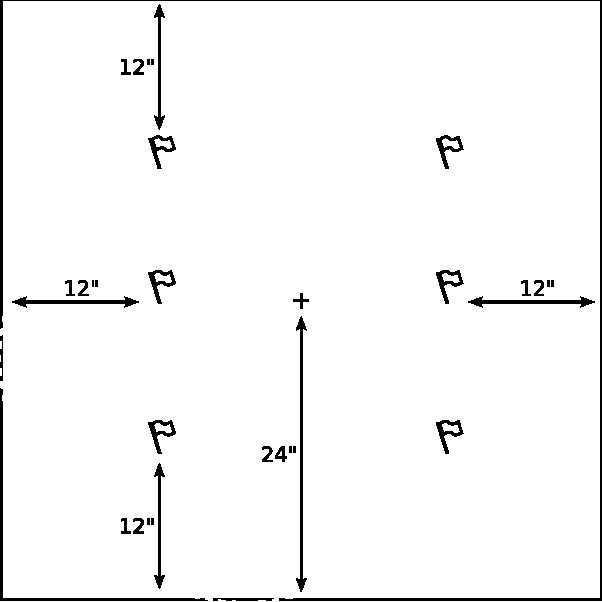
\includegraphics[width=\linewidth]{missions/ground-placement}
  \end{minipage}
  \hfill\hbox to 0pt{}

\end{tablesetup}

%%----------------------------------------------
\begin{missionrules}

\bigskip
There are no rules specific to this mission.

\end{missionrules}


%%----------------------------------------------
\begin{scoring}

\begin{primaries}
  Before any Scout redeployments, both players secretly choose one of
  the following primary scoring mechanisms for themselves:

  \begin{itemize}
  \item {\textit{Continuous.}} Beginning with Turn~2, score~1 victory
    point at the end of each of your player turns for each primary
    objective marker you control.
  
  \item {\textit{End Game.}} At game end, score~3 victory points for
    each primary objective marker you control.
  
  \end{itemize}

  This selection is declared along with the choice of secondary
  objective, below, after Scout redeployments.  Remember that
  \underline{no more than 9 victory points may be earned toward
    primary objectives}.  
\end{primaries}

\end{scoring}

%%----------------------------------------------------------------------
%%----------------------------------------------------------------------
\missiontitle{Mission: Slaughter Zone}

\teaser{War is not clever strategies; war is killing.}

\begin{tablesetup}    
  \hammerandanvil
\end{tablesetup}

%%----------------------------------------------
\begin{missionrules}

\bigskip
There are no rules specific to this mission.

\end{missionrules}


%%----------------------------------------------
\begin{scoring}
  
\begin{primaries}
  At game end, each unit that has been eliminated, is falling back, is
  in reserve, or has at most~25\% of its starting models remaining is
  broken.  Earn~2 victory points per quartile if at least 25\%, 50\%,
  and 75\% of the opposing army by units is broken.  Earn~1 victory
  point per quartile if at least 25\%, 50\%, and 75\% of your army is
  not broken.  An additional victory point is earned by the player who
  has had a smaller percentage of the units in their army broken.  If
  one player has been completely eliminated, the opposing player gains
  an additional victory point.  \underline{No more than 9 victory
    points may be earned via this primary objective.}
\end{primaries}

\end{scoring}

%%----------------------------------------------------------------------
%%----------------------------------------------------------------------
\missiontitle{Mission: Maelstrom}

\teaser{Only the agile can dance on the winds of war.}

\begin{tablesetup}    
  \vanguardstrike

  \smallskip%
  Players roll off on~D6 and in that order alternate placing a single
  primary objective marker each until a total of~6 have been placed.
  Label the markers~1 through~6 as they are placed.
\end{tablesetup}

%%----------------------------------------------
\begin{missionrules}
\standingorders
\end{missionrules}


%%----------------------------------------------
\begin{scoring}
  
\begin{primaries}
  \maelstromscoring
\end{primaries}

\end{scoring}

\clearpage
\squelchbackground
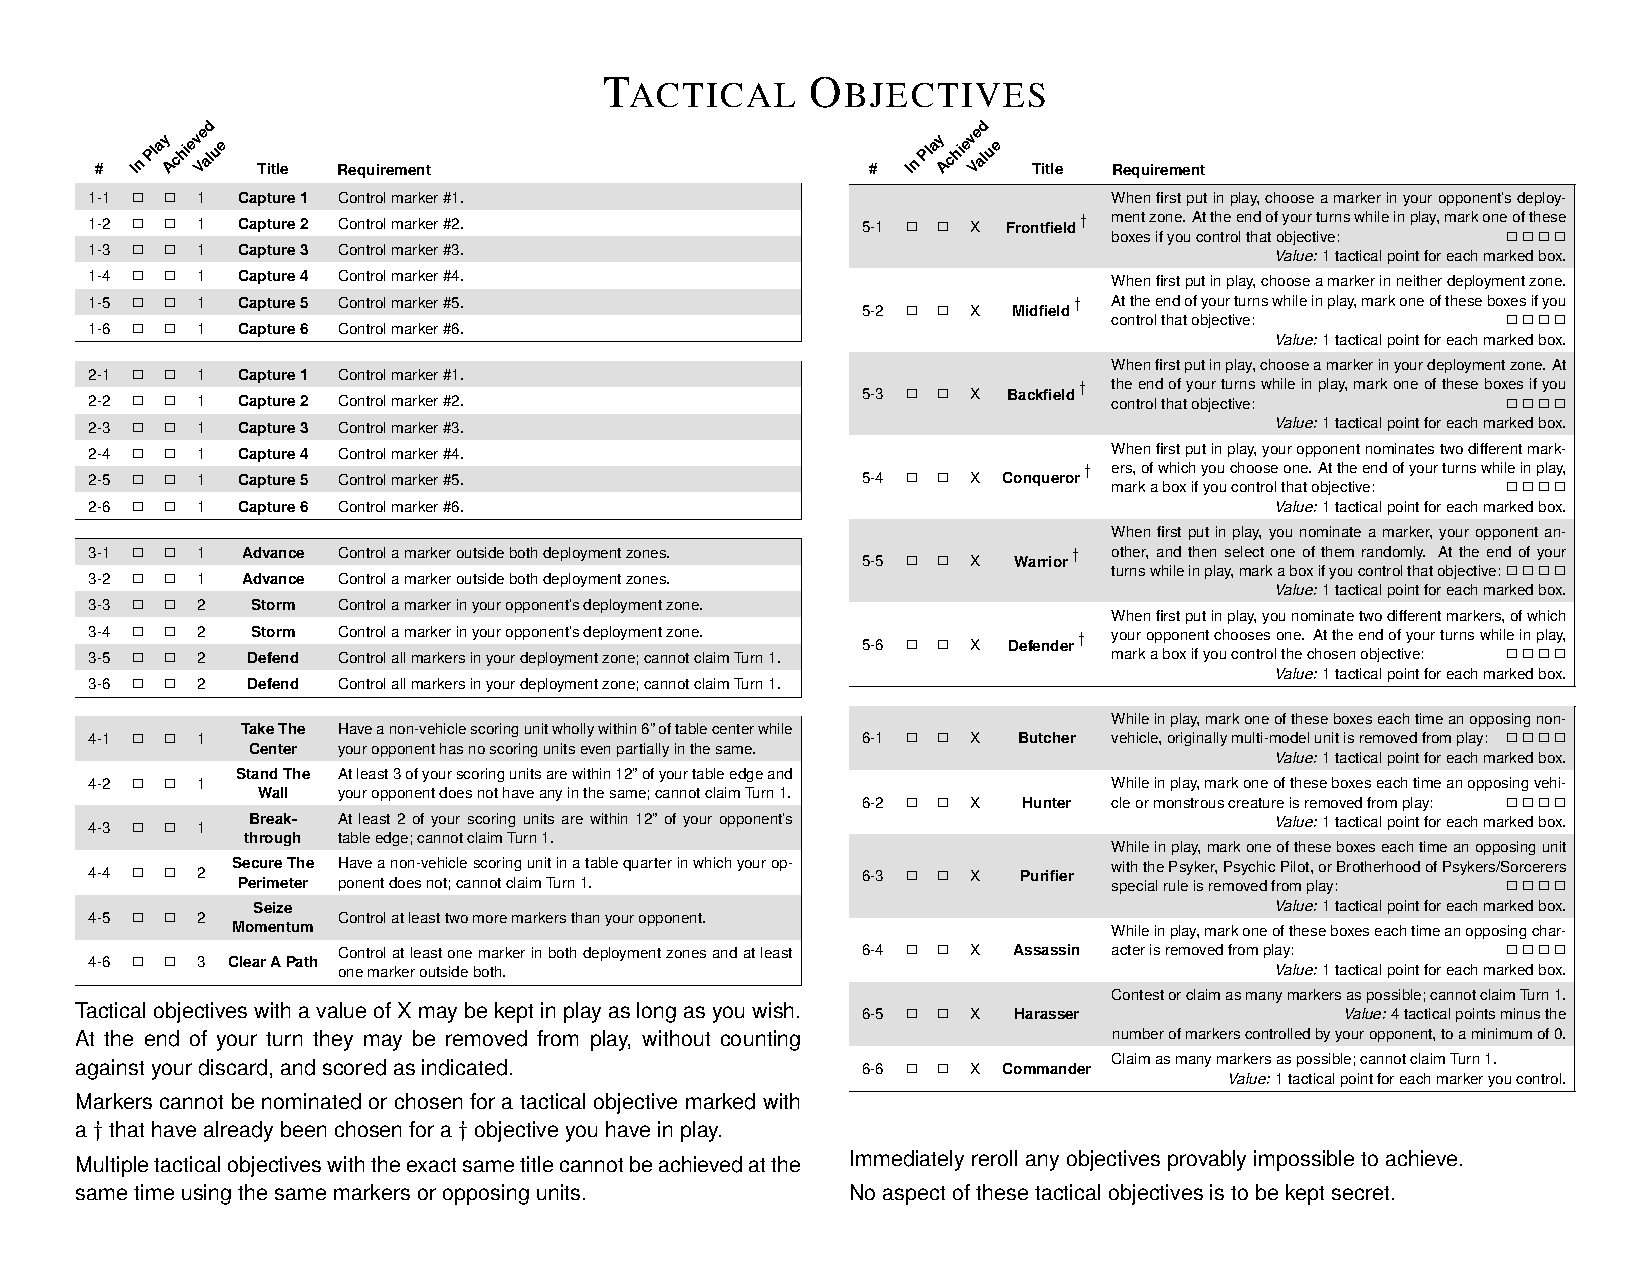
\includepdf[pages={1},fitpaper,offset=0cm 0cm]{tactical-objectives}
\pagebreak
\restorebackground



%%----------------------------------------------------------------------
%%----------------------------------------------------------------------
\begin{storyquotepage}  
  Who could have guessed this age, its unprecedented discord and
  dissent, would start with one small, unremarkable blue planet,
  itself already all but forgotten?

\bigskip
- Premiere Thyx,\\Transcripts of Governance Enclave TTTLAV.O
\end{storyquotepage}
%%----------------------------------------------------------------------
%%----------------------------------------------------------------------

\clearpage
\squelchbackground
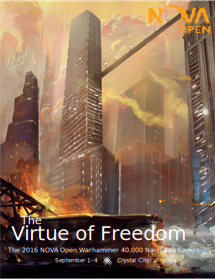
\includepdf[pages={1},fitpaper,offset=0cm 0cm]{art/back/back}
\pagebreak
\restorebackground

%\chapter{Timeline}

\end{document}

Three paths:

The Path of Daggers

Even the smallest of daggers can cause the gravest of wounds if they
come from behind.

- Attribution lost, The Chronicle of Foundation, sealed historical draft


The Path of Stone

Like a builder who cares only of paint colors, the enclaves too easily
forget the beings, the planets that are the stone foundations of our
society.

- Philosopher-in-exile 


The Path of Blood

War is easy.  Like fighting a v\"o, you cut out the heart and watch
the blood run out.

- Commandant P'Tika





The Virtue
The Coalition of the Free, or The Free as they're more popularly known.

Icons

Virtue: Couple dots, radar-ish circles

Free: Arrows in all directions


Daggers: There's a traitor among the Virtue.  Capture/protect or eliminate

Stone: Control the planets of the sector, by making the population happy or
conquering territory

Blood: Find the rebel base


Final round: Either or both of fighting to take over the Bend station,
or the rebel base

Dagger path pushes toward fighting the bend station
Blood path pushes toward fighting the rebel base
Stone path provides oomph toward either
